\documentclass[a4paper]{article}
\usepackage[utf8]{inputenc}
\usepackage[english]{babel}
\usepackage{gensymb}
\usepackage{textcomp}
\usepackage{graphicx}
\usepackage{rotating}
\usepackage{fancyhdr}
\usepackage{amsmath}
\usepackage{amsfonts}
\usepackage{siunitx}
\usepackage{listings}
\usepackage{color}
\usepackage{pbox}
\usepackage{tikz}
\usepackage{float}
\usepackage{drawstack}
\usepackage{booktabs}

\usetikzlibrary{shapes.geometric, shapes.multipart, arrows, svg.path}

\tikzstyle{startstop} = [rectangle, rounded corners, minimum width=3cm, minimum height=1cm,text centered, draw=black, fill=red!30]
\tikzstyle{io} = [trapezium, trapezium left angle=70, trapezium right angle=110, minimum width=3cm, minimum height=1cm, text centered, draw=black, fill=blue!30]
\tikzstyle{process} = [rectangle, minimum width=3cm, minimum height=1cm, text centered, draw=black, fill=orange!30]
\tikzstyle{decision} = [diamond, minimum width=3cm, minimum height=1cm, text centered, draw=black, fill=green!30]
\tikzstyle{arrow} = [thick,->,>=stealth]



\lstset{language=Python,
    backgroundcolor=\color{red!10},
    basicstyle=\color{black},
    keywordstyle=\color{blue},
    stringstyle=\color{purple},
    postbreak=\mbox{\textcolor{red}{$\hookrightarrow$}\space},
    commentstyle=\color{red},
    frame=single,
    numbers=left,
    showspaces=false,
    showstringspaces=true,
    breaklines=true}

\title{AlDa Script for the Summer Term 2018}
\author{Daniel Barley}

\pagestyle{fancy}
\fancyhf{}
\lhead{Alda}
\rhead{ST18}
\rfoot{Page \thepage}

\usepackage{hyperref}

\begin{document}

\maketitle

\tableofcontents

\newpage

\section{First lecture}
\begin{huge}
    Moodle PW: iad18
\end{huge}
\subsection{Introduction}
\subsubsection{What is an algorithm?}
\begin{itemize}
    \item an algorithm solves concrete problems and has to be:
        \begin{itemize}
            \item finite: it has to able to solve the problem with finite resources and in finite steps.
            \item terminal: it has to terminate after a finite time.
            \item determinism: it has to give the same output when given the same input.
            \item analyzable: runtime and memory usage are predictable.
            \item correctness: it should be possible to check weather the algorithm solves the problem corectly.
        \end{itemize}
\end{itemize}
\subsubsection{An example}
\begin{itemize}
    \item calculating the factorial:
        \begin{itemize}
            \item definition $ N! = N (N-1)(N-1) \dots 1 $
        \end{itemize}
    \item two possible solutions:
        \begin{itemize}
            \item loop
            \item recursion
        \end{itemize}
\end{itemize}
\begin{lstlisting}
def Fak(N):
    for i in range(N + 1):
        fa = fa * i
    return fa
\end{lstlisting}

\begin{lstlisting}
def Fak(N):
    if N == 1:
        return 1
    else:
        return N * Fak(N - 1)
\end{lstlisting}
\subsubsection{General workflow:}
\begin{itemize}
    \item Specify the problem
    \item Create an algorithm
    \item Look for the most efficient solution
    \item Convert into elementary steps (implement in a programming language)
\end{itemize}
\subsubsection{Classification of algorithms}
\begin{itemize}
    \item iterative algorithms:
        \begin{itemize}
            \item sequence of operations is predetermined.
        \end{itemize}
    \item recursive algorithms:
        \begin{itemize}
            \item break problem into simpler sub problems
            \item special treatment for trivial case.
        \end{itemize}
\end{itemize}

\section{Second Lecture}
\subsection{Turing Machine}

\begin{itemize}
    \item Proposed by Alan Turing
    \item Consists of a Control Unit with a write/read head and an internal memory
    \item the memory is realized by an infinite band of paper
    \item the instrucctional set consits of
        \begin{itemize}
            \item read
            \item write
            \item move to the right (by $n$ cells)
            \item move to the left (by $n$ cells)
            \item goto a specific cell
            \item if \texttt{'a'} on memory cell goto $ k $ if not goto $ l $
            \item stop
        \end{itemize}
\end{itemize}

\subsection{Turings Thesis}

\begin{itemize}
    \item The set of Turing-computable Problems is equivalent to the set of intuitively computable Problems
        \begin{itemize}
            \item examples of non computable Problems:
                \begin{itemize}
                    \item Halting Problem (check weather Truing code ever halts)
                    \item Correctness Problem (does a Turing machine compute a desired function)
                    \item Equivalency Problem (do two Turing Machines compute the same function)
                \end{itemize}
        \end{itemize}
\end{itemize}

\subsection{Analysis of algorithms}
A simple example:
\begin{itemize}
    \item sorting Numbers. Some questions arise:
        \begin{itemize}
            \item is the algorithm correct
            \item how much memory is needed
            \item how much time is needed
            \item how accurate is the solution, what bandwidth is needed
        \end{itemize}
\end{itemize}

\subsubsection{Correctness}
\begin{itemize}
    \item Induction:
        \begin{itemize}
            \item $ A $ over the naturals $ n \in \mathbb{N}$ %$ A(n) $
                \begin{itemize}
                    \item start: show that $ A(1) $ is correct
                    \item step: show that when going from $ A(n) \Rightarrow A(n +1) $ it still holds correct
                \end{itemize}
        \end{itemize}
    \item Invariants
        \begin{itemize}
            \item loop invariants are constants that do not change in the scope of the loop
        \end{itemize}
    \item Tests
\end{itemize}

\subsubsection{Complexity}
\begin{itemize}
    \item get the number of needed operations
    \item Simple description independent from computer and quality of code
    \item analyze behavior in different cases
        \begin{itemize}
            \item best case
            \item average case
            \item worst case
        \end{itemize}
\end{itemize}
The goal is not to give an exact ETA but to give some guidelines for scalability.
Since the average case is hard to guess most analysis consists of best/worst case analysis.

Example

\begin{table}[htpb]
    \centering
    \caption{Example}
    \label{tab:label}
    \begin{tabular}{cccc}
        n & 1 & 100 & 1000 \\
        $ T(n)=n $ & 1 & 10 & 1000 \\
        $ T(n)=n^2 $ & 1 & 100 & 10000 \\
        $ T(n)=2^n $ & 2 & $ \approx  10^3 $ & $ \approx  10^{30} $
    \end{tabular}
\end{table}

\subsection{principles of algorithms}
\subsubsection{Enumeration}
List all the possible solutions.

Example:
\begin{itemize}
    \item Maximum-Subarray-Problem:
    \item given the series of reels $ a _{n}, a _{1}, \dots a _{n-1} \in \mathbb{R}  $
    \item look for consecutive of length $ R $ series of elements with maximum partial sum
    \item example: $ 31, 41, \underbrace{59, 26, 53, 58, 97}_{187} , 93, 23, 84 $
\end{itemize}

Two simple solution:
\begin{lstlisting}
def maxSubarray(A, n):
    maxsum = 0
    for L in range(n):
        for R in range(L, n):
            sum = 0
            for i in range(L, R):
                sum = sum + A[i]
            if sum > maxsum:
                maxsum = sum
    return maxsum
\end{lstlisting}

Other solution:

\begin{lstlisting}
def maxSubarray(A, n):
    maxsum = 0
    for L in range(n):
        sum = 0
        for R in range(L, n):
            sum = sum + A[i]
            if sum > maxsum:
                maxsum = sum
    return maxsum
\end{lstlisting}

\subsubsection{Divide and Conquer}
\begin{itemize}
    \item divide the problem in to simpler subproblems until a trivial case is reached
    \item solve the trivial case
    \item reconstruct the Solution from solved subproblems
\end{itemize}
Most of the time the complexity is around $ T(n) \approx n \log_2 n $

\subsubsection{Scanline-Method}

\begin{itemize}
    \item simple scanning of the array
\end{itemize}

Example:
Isosurfaces: given a lettuce( :) ) of points find surfaces by scanning point wise intensity

\newpage

\section{Third Lecture}

\subsection{simple data structures}
\begin{itemize}
    \item Algorithms
        \begin{itemize}
            \item efficiency
                \begin{itemize}
                    \item complexity:
                        merit for computing time / memory usage
                \end{itemize}
        \end{itemize}
    \item Data strucutres
        \begin{itemize}
            \item efficient access
            \item operations on data strucutres
                \begin{itemize}
                    \item need fast algorithms
                \end{itemize}
        \end{itemize}
    \item Abstract data type
        \begin{itemize}
            \item specification of what kind of data is stored
            \item specification of the kind of operations performed on the structure
        \end{itemize}
    \item Data strucutres
        \begin{itemize}
            \item implementation of abstract datatypes
            \item maybe different complexities / runtimes
        \end{itemize}
\end{itemize}
examples:
\begin{itemize}
    \item arrays
    \item lists
    \item stacks
    \item queue
\end{itemize}

\subsubsection{Arrays}
\begin{itemize}
    \item predefined in most languages
    \item used for
        \begin{itemize}
            \item vectors, matrices, images, \dots
            \item numerics, image processing
        \end{itemize}
    \item properties
        \begin{itemize}
            \item selection of congruent elements
            \item access via index
        \end{itemize}
    \item most of the time arrays are statically defined (fixed sized)
    \item generalization
        \begin{itemize}
            \item stacks, queues, dynamic arrays
        \end{itemize}
\end{itemize}
The array as an abstract datatype holds elements of the same datatype.
There are some necessary operations an array has to have:
\begin{itemize}
    \item \texttt{create (n)}: creates an array of size \texttt{n}
    \item \verb&A.get(i)&: returns element at position \texttt{i}
    \item \verb&A.set(x, i)&: write \texttt{x} to position \texttt{i}
    \item \verb&A.size()&: returns length of array
\end{itemize}
A dynamic array has to also have the following methods:
\begin{itemize}
    \item \verb&A.append(x)&: creates a new entry with value \texttt{x} at the end
    \item \verb&A.pop(x)&: deletes the last element
\end{itemize}
example \texttt{vector} of the \emph{C++ standard library} internally allocates, in the simplest case, double the amount of memory.
So that at most $ k \log{n} $ accesses are needed, and at most $ k \cdot n $ memory is wasted

SIDENOTE: Computer architecture
\begin{itemize}
    \item CPU
        \begin{itemize}
            \item program memory: list of operations
            \item data storage: data
            \item most simple model: sequential computation of operations obtained from the program memory
            \item faster: pipelining: divide the operation into smaller parallel instructions like:
                \begin{itemize}
                    \item fetch
                    \item instruction decode
                    \item execute
                    \item mempry
                    \item write back
                \end{itemize}
            \item even faster: multi scalar: local parralelisation
            \item now: multicore: multiple CPUs on one die.
        \end{itemize}
\end{itemize}
good algorithms make good use of architecture.
\begin{itemize}
    \item Memory
        \begin{itemize}
            \item hard drive, SSD: good for large amounts of data but slow access
            \item memory (DRAM): faster
            \item cache hierarchy
                \begin{itemize}
                    \item very fast access, if data is accesses in time wise order
                    \item third level cahce (SRAM)
                    \item second level cahce
                    \item first level cache
                \end{itemize}
        \end{itemize}
\end{itemize}
good algorithms make good use of memory hierarchy (caching)

\begin{itemize}
    \item \framebox[1.1\width]{Register}
    \item \framebox[1.1\width]{1st level cache}
    \item \framebox[1.1\width]{2nd level cache}
    \item \framebox[1.1\width]{3rd level cache}
    \item \framebox[1.1\width]{RAM}
    \item \framebox[1.1\width]{Hard drive}
\end{itemize}

\subsubsection{lists}
\begin{itemize}
    \item multiple sets of data (maybe of different type)
    \item access is serial, ideally only operations on neighboring elements
    \item appending is easy
        \begin{itemize}
            \item append at the end
            \item append as first element
            \item middle: append by changing pointers to following elemnts
        \end{itemize}
    \item cons
        \begin{itemize}
            \item very slow when not operating serially on neighbors
        \end{itemize}
\end{itemize}
example:
\begin{lstlisting}
class listElement:
    def __init__(self,
                key=0,
                data=None,
                next=None,
                prev=None):
        self.key = key
        self.data = data
        self.next = next
        self.prev = prev
\end{lstlisting}
different flavours of lists include:
\begin{itemize}
    \item single chained lists: each element has a reference to its successor
    \item double chained lsits: each element has a reference to bot its successor and predecessor
\end{itemize}
example for search with a list:
\begin{lstlisting}
current = first
while current != None and current_key != x:
    current = current_next
\end{lstlisting}
is of complexity $ \mathcal{O}(n) $

\section{Fourth Lecture}
\subsection{Stacks and Queues}
\begin{itemize}
    \item Stack
        \begin{itemize}
            \item \verb%create()% creates an empty stack
            \item \verb%stack.push(a)% appends element to the "top" of the stack
            \item \verb%stack.pop()% deletes the "top" element
            \item \verb%stack.peek()% looks up the "top" element, without changing it
            \item \verb%stack.is_empty()% returns \verb%true% if the Stack is empty
            \item The Stack is a "LIFO" (Last In First Out) memory
        \end{itemize}
    \item Queue
        \begin{itemize}
            \item \verb%queue.enqueue(a)% appends at the "top"
            \item \verb%queue.dequeue()% returns first element and removes it
            \item \verb%queue.is_empty()% returns \verb%true% if the Stack is empty
            \item The Queue is a "FIFO" (First In First Out) memory
        \end{itemize}
\end{itemize}
A special form of the queue is the priority queue which stores key value pairs and supports the following operations
\begin{itemize}
    \item \verb%pqueue.create()% creates an empty priority queue
    \item \verb%pqueue.insert(x, key)% inserts a key value pair
    \item \verb%pqueue.getMin()% returns the element with the smallest key assigned
    \item \verb%pqueue.deleteMin()% removes the element with the smallest key assigned
    \item analogous to the \texttt{Min} these two methods can be implemented for the largest keys respectively
\end{itemize}
The most common implementation of the priority queue is the heap

\subsubsection{Stack/Queue Schematics}
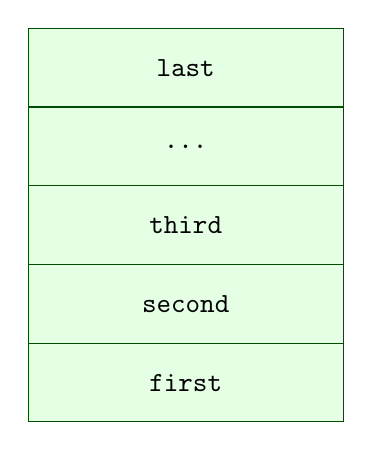
\begin{tikzpicture}
    \cell{\texttt{last}};
    \cell{\texttt{\dots}};
    \cell{\texttt{third}};
    \cell{\texttt{second}};
    \cell{\texttt{first}};
\end{tikzpicture}

Note that first denotes the first element on the stack/queue time wise \dots.

\subsubsection{\texttt{stack.peek()}}

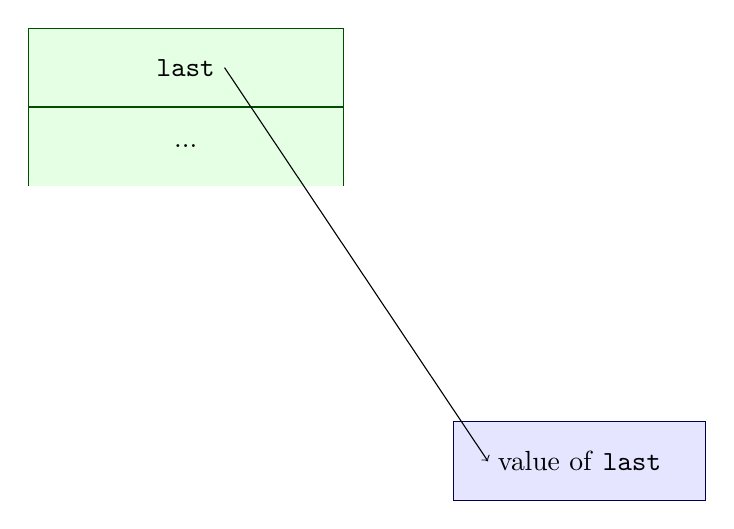
\begin{tikzpicture}
    \cell{\texttt{last}} \coordinate (last) at (currentcell.east);
    \stackbottom;
    \drawstruct{(5, -5)};
    \structcell{value of \texttt{last}} \coordinate (return) at (currentcell.west);
    \draw[->] (last) -- (return);
\end{tikzpicture}

\subsubsection{\texttt{stack.pop()}}

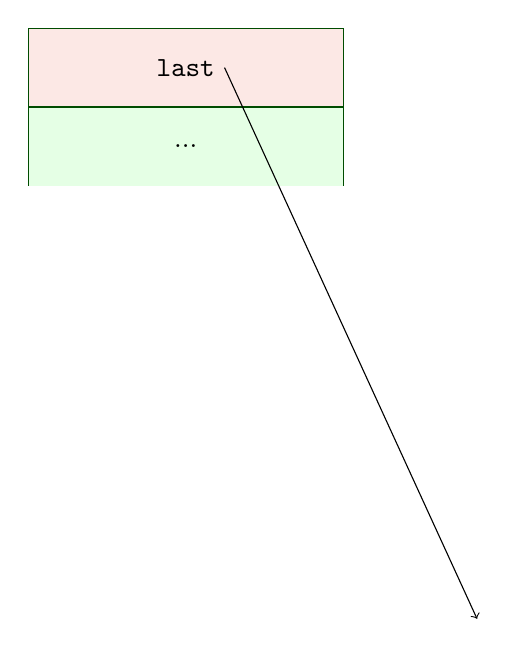
\begin{tikzpicture}
    \bcell{\texttt{last}} \coordinate (last) at (currentcell.east);
    \stackbottom;
    \draw[->] (last) -- (3.7, -8);
\end{tikzpicture}

\subsubsection{\texttt{stack.push()}}

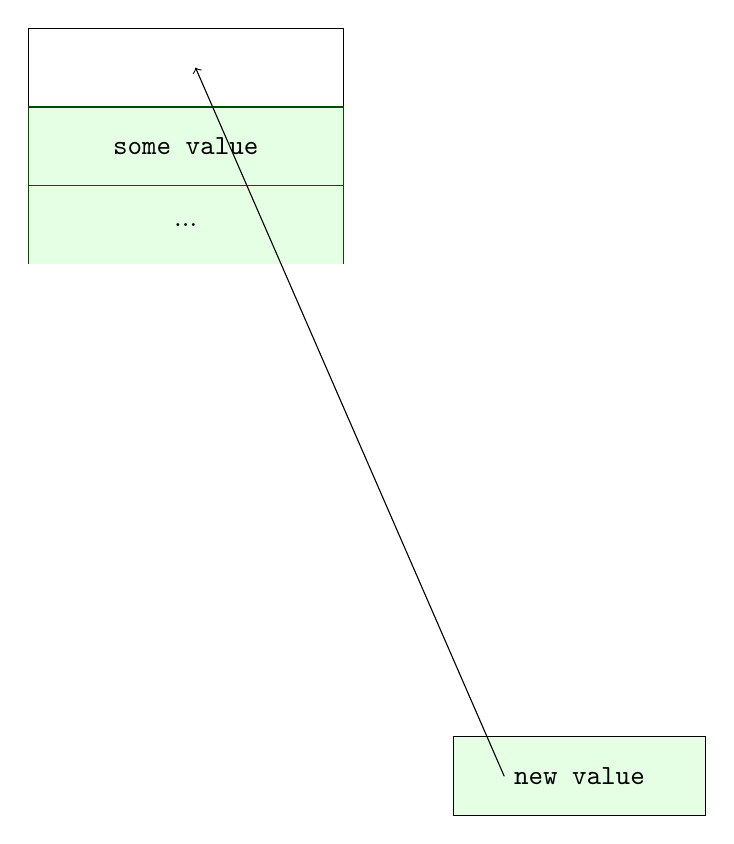
\begin{tikzpicture}
    \cell[color=black, fill=white]{\texttt{}} \coordinate (some) at (currentcell.east);
    \cell{\texttt{some value}};
    \stackbottom;
    \drawstruct{(5, -9)};
    \structcell[color=black, fill=green!10]{\texttt{new value}} \coordinate (new) at (currentcell.west);

    \draw[<-] (some) -- (new);
\end{tikzpicture}

\subsubsection{\texttt{queue.enqueue}}
same as \texttt{stack.push()}

\subsubsection{\texttt{queue.dequeue}}

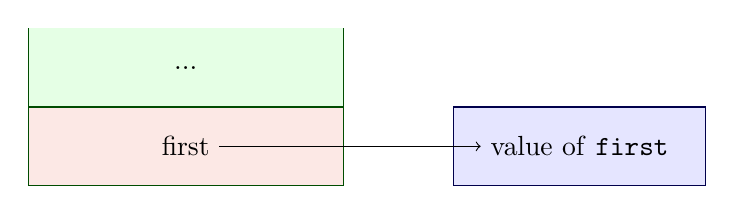
\begin{tikzpicture}
    \stacktop{}
    \bcell{first} \coordinate (first) at (currentcell.east);
    \drawstruct{(5, 0)};
    \structcell{value of \texttt{first}} \coordinate (return) at (currentcell.west);
    \draw[->] (first) -- (return);
\end{tikzpicture}

\subsubsection{Priority Queue}

\begin{drawstack}
    \cell{\texttt{someValue}} \cellcom{ $ i $ };
    \cell{\texttt{someOtherValue}} \cellcom{ $ j $ };
\end{drawstack}

\subsubsection{\texttt{pqueue.insert()}}

\begin{drawstack}
    \cell{\texttt{someValue}} \cellcom{ $ i $ };
    \cell[color=black, fill=white]{} \coordinate (empty) at (currentcell.east);
    \cell{\texttt{someOtherValue}} \cellcom{ $ j $ };
    \drawstruct{(5, -1)};
    \structcell[fill=green!10]{\texttt{someNewValue}} \coordinate (new) at (currentcell.west);
    \draw[<-] (empty) -- (new);
    \draw (8.5, -2) node (bla){
        \begin{tabular}{c}
            $ k $ with $ i < k < j $
        \end{tabular}
    };
\end{drawstack}

\subsection{Dictionaries (or Maps, Associative Arrays)}
A dictionary holds a set of elements each assigned an unambiguous key
Instead of an access through an index dictionaries are accessed via the element's key.
The following operations are possible:
\begin{itemize}
    \item \verb%dict.create()% creates an empty dict
    \item \verb%dict.insert(x, key)% add a value key pair
        \begin{itemize}
            \item if the key already exists it will be overridden
        \end{itemize}
    \item \verb%x = dict.find(key)% returns the entry \texttt{x}
        \begin{itemize}
            \item if the key is non existent return a default value
        \end{itemize}
    \item \verb%dict.delete(key)% removes value belonging to the respective key
\end{itemize}

\begin{table}[H]
    \centering
    \caption{Complexity}
    \label{tab:label}
    \begin{tabular}{ccccc}
        \toprule \\
        operation       & list               & array              & sorted array            & dictionary                 \\
        \midrule \\
        \texttt{create} & $ \mathcal{O}(1) $ & $ \mathcal{O}(1) $ & $\mathcal{O}(1) $       & $ \mathcal{O}(1) $         \\
        \texttt{insert} & $ \mathcal{O}(n) $ & $ \mathcal{O}(n) $ & $\mathcal{O}(n) $       & $ \mathcal{O}(n \log{n}) $ \\
        \texttt{find}   & $ \mathcal{O}(n) $ & $ \mathcal{O}(n) $ & $\mathcal{O}(\log{n}) $ & $ \mathcal{O}() $          \\
        \texttt{delete} & $ \mathcal{O}(n) $ & $ \mathcal{O}(n) $ & $\mathcal{O}(n) $       & $ \mathcal{O}() $          \\
        \bottomrule
    \end{tabular}
\end{table}

\subsection{Sorting}
\subsubsection{Motivation}
sorting is one of the most common problems (approx. $ \frac{1}{4} $ of the total computing time)
\subsubsection{Problem}
Given a sequence of $ n $ elements $ x _{1}, x _{2} , \dots, x _{n} $, the $ > $ and $ < $ relations have to be defined and $ x _{i} \leq x _{j} $ should give a boolean (\texttt{true/false}).
The result should be a sorted sequence i.e $ \forall i < j \Rightarrow x_{i} \leq x _{j} $.
This for example be achieved by permutation (series of swaps).
\subsubsection{Selection Sort}
The selection sort algorithm is a very simple one, it consists of the following steps:
\begin{itemize}
    \item find the smallest element
    \item swap with the first element
    \item continue
\end{itemize}
An example implementation:

\begin{lstlisting}
def selectionSort(alist):
    for i in rage(len(alist) - 1):
        least = i
        for k in range(i + 1, len(alist)):
            if alist[k] < alist[least]:
                least = k
                temp = alist[least]
        alist[least] = alist[i]
        alist[i] = temp
\end{lstlisting}

\subsubsection{Insertion Sort}
The insertion sort algorithm is often used by humans when playing card games.
\begin{itemize}
    \item start with the second element
    \item check if it is greater than the first
    \item if so swap the element to the left until smaller than next element
    \item then continue with the third element
    \item repeat until sorted
\end{itemize}
we can divide the array into two parts:
\begin{itemize}
    \item presorted start
    \item not yet sorted end
\end{itemize}

\begin{lstlisting}
def insertionSort(alist):
    for index in range(1, len(alist)):
        current_value = alist[index]
        position = index
        while position > 0 and alist[psition - 1] > current_value:
            alist[position] = alist[position - 1]
        alist[position] = current_value
\end{lstlisting}

\subsection{SIDENOTE: how to record runtime in Python}
\begin{lstlisting}
    import time

    start_time = time.time()
    run_time = (time.time() - start_time) * 1000 #because time returns microseconds
\end{lstlisting}

\section{Fifth Lecture}

\subsection{Bubble Sort}

\begin{itemize}
    \item look through array until two values are not sorted, correct that
    \item repeat until completely sorted
    \item array is sorted from back to front, i.e first the largest element is pushed to the back
\end{itemize}

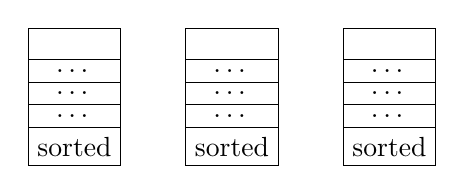
\begin{tikzpicture}[stack/.style={rectangle split, rectangle split parts=#1,draw, anchor=center}]
    \node[stack=5] at (0, 0)  {
    \nodepart{two}\dots
    \nodepart{three}\dots
    \nodepart{four}\dots
    \nodepart{five}sorted
};
    \node[stack=5] at (2, 0)  {
    \nodepart{two}\dots
    \nodepart{three}\dots
    \nodepart{four}\dots
    \nodepart{five}sorted
};
    \node[stack=5] at (4, 0)  {
    \nodepart{two}\dots
    \nodepart{three}\dots
    \nodepart{four}\dots
    \nodepart{five}sorted
};
\end{tikzpicture}

\begin{lstlisting}
def bubbleSort(nlist):
    for j in range(len(nlist) -1):
        for i i range(nlist-i-j):
            if nlist[i] > nlist[i+1]:
                temp = nlist[i]
                nlist[i] = nlist[i+1]
                nlist[i+1] = temp
\end{lstlisting}

\newpage

\subsection{Divide and Conquer}
\subsubsection{Quick Sort}
\begin{itemize}
    \item choose an (ideally median) element from list as pivot
    \item create two lists and sort in elements accordingly
        \begin{itemize}
            \item left: smaller than pivot
            \item right: larger than pivot
            \item sort both sub lists
        \end{itemize}
\end{itemize}

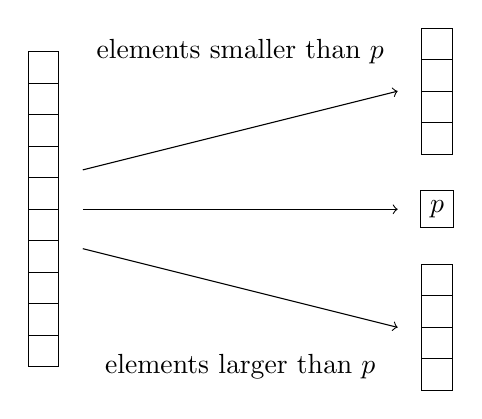
\begin{tikzpicture}[stack/.style={rectangle split, rectangle split parts=#1,draw, anchor=center}]
    \node[stack=10] at (0, 0)  {
    \nodepart{two}
    \nodepart{three}
    \nodepart{four}
    \nodepart{five}
    \nodepart{six}
    \nodepart{seven}
    \nodepart{eight}
    \nodepart{nine}
    \nodepart{ten}
};
\node[stack=4] at (5, 1.5)  {
    \nodepart{two}
    \nodepart{three}
    \nodepart{four}
    \nodepart{five}
    \nodepart{six}
    \nodepart{seven}
    \nodepart{eight}
    \nodepart{nine}
    \nodepart{ten}
};

\node[stack=1] at (5, 0) {
    \nodepart{one}$p$
};

\node[stack=4] at (5, -1.5)  {
    \nodepart{two}
    \nodepart{three}
    \nodepart{four}
    \nodepart{five}
    \nodepart{six}
    \nodepart{seven}
    \nodepart{eight}
    \nodepart{nine}
    \nodepart{ten}
};

\node at (2.5, 2){
    elements smaller than $p$
};

\node at (2.5, -2){
    elements larger than $p$
};

\draw[->] (0.5, 0) -- (4.5, 0);
\draw[->] (0.5, 0.5) -- (4.5, 1.5);
\draw[->] (0.5, -0.5) -- (4.5, -1.5);
\end{tikzpicture}

\begin{itemize}
    \item divide problem into (two or more) sub problems
    \item recursively solve those sub problems
    \item combine sub solutions to solve the initial problem
\end{itemize}
How to pivot the array:
\begin{itemize}
    \item go through array from left to right
    \item if the element's index and value are smaller than the pivot do nothing
    \item if not swap with an element from the other side
    \item take $ l $ and $ r $ to walk through the array from left to right ( $ l $ ) or from right to left ( $ r $ )
    \item increment $ l $ until $ A[ \ l \ ] > p $ (this element has to be swapped to the right) 
    \item decrement $ r $ until $ A [ \ r \ ] \leq p $ (this element has to be swapped)
    \item swap element $ l $ with $ r $ 
    \item $ l = l + 1 $ and $ r = r-1 $ 
    \item done when $ l = r $ 
\end{itemize}
Note that choice matters when it comes to the pivot.
Ideally the pivot splits the list into two parts, almost equal in size.
But Since calculating the median requires sorting simply choosing the median is not an option.
In reality some random element is often chosen as pivot, like the first or last element or a random choice.
For more precision an assortment of elements can randomly be selected from the list.
The pivot is then obtained by choosing the median of those elements.

Even though quick sort is somewhat fast (of average complexity $ \mathcal{O}(n \cdot \log{n}) $)
it has one problem. Choosing an inefficient pivot (deviating a lot from the median) adds a lot of complexity.

\subsubsection{Merge Sort}
Merge Sort avoids quick sort's pivot problems by not using one.
\begin{itemize}
    \item divide list in the middle
    \item recursively sort the sub lists
    \item combine sorted sub lists
\end{itemize}

\section{Sixth Lecture}
\subsection{Merge Sort revisited}
\begin{table}[H]
    \centering
    \caption{Quicksort vs. Mergesort}
    \label{tab:sorting}
    \begin{tabular}{cc}
        \toprule \\
        Quicksort & Mergesort \\
        \midrule \\
        $ \mathcal{O}(n \cdot \log{n}) $ on average & $ \mathcal{O}(n \cdot \log{n}) $ on average \\
        $ \mathcal{O}(n^2) $ in worst case & $ \mathcal{O}(n \cdot \log{n}) $ in worst case \\
        \bottomrule
    \end{tabular}
\end{table}

\begin{lstlisting}
MergeSort(A, start, end, tmp):
    if end - start > 1:
        middle = start + (end - start) // 2 #integer division
        MergeSort(A, start, middle, tmp)
        MergeSort(A, middle, end, tmp)
    pos = start
    i = start
    j = middle
    while pos < end:
        if(i < middle) and (j = end) or (A[i] < A[j]):
            tmp[pos] = A[i]
            i += 1
            pos += 1
        else:
            tmp[pos] + A[j]
            j += 1
            pos += 1
\end{lstlisting}
So merge Sort is guaranteed to be of complexity $ n \cdot \log{n} $. 

\subsection{Complexity}
\begin{itemize}
    \item How does the computing time change with respect to the problem's size?
    \item different possible approaches for merit
        \begin{itemize}
            \item simply measure computing time
                \begin{itemize}
                    \item depends on the used hardware
                    \item depends on implementation and programming language
                \end{itemize}
            \item count the number of elementary operations
                \begin{itemize}
                    \item better approximation
                    \item still deviations on real systems (caching)
                \end{itemize}
        \end{itemize}
\end{itemize}
The complexity is an abstract merit for runtime predictions.
A naive approach would be to simply count the number of atomic operation needed to complete the task at hand.
For example:
\begin{itemize}
    \item $ +, -, /, *, \% $ 
    \item memory access
    \item function calls
\end{itemize}
For this to be consistent some approximations have to be made:
\begin{itemize}
    \item all atomic operations cost exactly one unit of time
    \item all memory access is equally fast
\end{itemize}
\subsubsection{example: Insertion Sort}
\begin{table}[H]
    \centering
    \caption{Atomic Operations Insertion Sort}
    \label{tab:insertion}
    \begin{tabular}{lcc}
        \toprule \\
        insertionSort(A) & cost & number of calls \\
        \midrule \\
        \verb#for j=2 to A.lenght# & $ C_1 $ & $ n $ \\
        \verb#key = A[i]# & $ C_2 $ & $ n-1 $ \\
        \verb#i = j-1# & $ C_4 $ & $ n-1 $ \\
        \verb#while j > 0 and a[i] > key# & $ C_5 $ & $ \sum_{j=2}^{n} t $ \\
        \verb#    A[i+i] = A[i]# & $ C_6 $ & $ \sum_{j=2}^{n} (t_j -1) $ \\
        \verb#    i = j - 1# & $ C_7 $ & $ \sum_{j=2}^{n} (t_i -1) $ \\
        \verb#A[i + j] = key# & $ C_8 $ & $ n-1 $ \\
        \bottomrule
    \end{tabular}
\end{table}
\subsubsection{Further Simplification}
Example:
\begin{itemize}
    \item Runtime is given by $ T(n) = a n^2 + b n + c $ 
    \item The parameters $ a, b, c $ still depend on the implementation and the hardware
\end{itemize}
In order to obtain a hardware independent estimate we drop all parameter and only take the fastest growing term into account.
\begin{itemize}
    \item up until now: look at the number of atomic operations
        \begin{itemize}
            \item simplification 1: calculate upper limit by counting atomic operations
            \item Simplification 2: parameter is size of input $ n $ 
        \end{itemize}
\end{itemize}

\subsection{Bachmann-Landau Notation or Big-O Notation}
Using the Big-O notation the asymptotic behavior of functions can be approximated.
\begin{itemize}
    \item $ \exists C $ so that $ C:T(n) \leq Cf(n) \Rightarrow T(n) \in \mathcal{O}(f(n)) $ 
    \item $ \exists C' $ so that $ C' T(n) \geq C'f(n) \Rightarrow T(n) \in \Omega(f(n)) $ 
\end{itemize}
formal definitions:
\begin{itemize}
    \item $ \mathcal{O}(f(n)) = \{f \  | \ \exists C > 0, n_0 > 0 \  \forall n \geq n_0 : f(n) \leq g(n)\} $ 
    \item $ f(n) \in \mathcal{O}(g(n)) $, if there exists constant $ C > 0, n_0 >0 $ so that $ f(n) \leq C g(n) $ for all $ n \geq n_0 $ 
    \item $   \Omega(f(n)) = \{f \  | \ \exists C > 0, n_0 > 0 \  \forall n \geq n_0 : f(n) \geq g(n)\} $ 
    \item $ f(n) \in \mathcal{O}(g(n)) $, if there exists constant $ C > 0, n_0 >0 $ so that $ f(n) \geq C g(n) $ for all $ n \geq n_0 $ 
    \item in short:
    \item $ f(n) \in \mathcal{O}(g(n)) $ 
        \begin{itemize}
            \item $ f(n) $ does not grow faster than $ g(n) $ (asymptotically) 
        \end{itemize}
    \item $ f(n) \in \Omega(g(n)) $ 
        \begin{itemize}
            \item $ f(n) $ does grow at least as fast as $ g(n) $ (asymptotically) 
        \end{itemize}
\end{itemize}

\subsubsection{Example Bubble Sort}
Pseudo-Code:
\begin{lstlisting}
BubbleSort(A):
    for i in range(0, n-2):
        for j in range(0, n-2-i):
            if A[j] > A[i+j]:
                swap(A[j], A[j+1])
\end{lstlisting}
$ T(n) \leq c \underbrace{\# \text{loop count}}_{X(n)} $ 
so $ c' n^2 \leq X(n) = \sum_{i=0}^{n-2} (n-2-i) \leq c n^2 $ therefore $ T(n) \in \mathcal{O}(n^2) $ with 
$ T(n)= \begin{cases}
    f(n) \in \Omega(n^2) \\
    f(n) \in \Theta(n^2)
\end{cases} $ 




\end{document}
